\chapter{Refactoring}

\section{Code Smells}

\subsection*{}
\vspace{0.5cm}
\begin{lstlisting}[caption={Code Smell I (Vorher)}]
    @Override
    public void move(Direction direction) {
        RoomPosition target = this.getPosition().getAdjacentPosition(direction);
        if (target.isValid() && target.isFree()) {
            if (this.getRoom() instanceof BossRoom boss) {
                RoomPosition trapdoor = boss.getTrapdoorPosition();
                
                if (target.equals(trapdoor) && this.getRoom().isCleared()) {
                    this.game.nextLevel();
                }
            }
            
            this.setPosition(target);
            
            Item underneath = this.getRoom().getItemUnderneath(this.getPosition());
            // this.game.setItemUnderneath(underneath);
        } else {
            if (!this.getRoom().isCleared()) {
                return;
            }
            
            this.getRoom().getDoors().forEach(door -> {
                if (door.getRoomPosition().equals(target)) {
                    this.game.getLevel().enter(door);
                }
            });
        }
    }
\end{lstlisting}

\vspace{0.5cm}
\begin{lstlisting}[caption={Code Smell I (Nachher)}]
    @Override
    public void move(Direction direction) {
        RoomPosition target = this.getPosition().getAdjacentPosition(direction);
        if (target.isValid() && target.isFree()) {
            if (this.getRoom().isBossRoom()) {
                RoomPosition trapdoor = this.getRoom().getTrapdoorPosition();
                if (target.equals(trapdoor) && this.getRoom().isCleared()) {
                    this.game.nextLevel();
                }
            }
            
            this.setPosition(target);
            
            Item underneath = this.getRoom().getItemAt(this.getPosition());
            // this.game.setItemUnderneath(underneath);
        } else {
            if (!this.getRoom().isCleared()) {
                return;
            }
            
            Door door = this.getRoom().getDoorAt(target);
            if (door != null) {
                this.game.getLevel().enter(door);
            }
        }
    }
\end{lstlisting}


\section{Refactorings}
\subsection{Rename Method}
Der erste Code und das erste UML-Diagramm zeigen den Zustand vor
dem Refactoring (Commit 3174f95). Dabei ist zu sehen, dass die \textit{place()}-Funktion
mit einer Liste namens \textit{fixedComponents} interagiert. Hier
scheint es um fixierte \textit{Buffer} zu gehen, was der Funktionsname
aber nicht zum Ausdruck bringt. Dabei ist \textit{place()} ein
Platzhaltername gewesen. Der Name ist nicht sonderlich aussagekräftig.
Es wird keine Aussage darüber getroffen, \textbf{wie} oder \textbf{unter
welchen Annahmen} ein \textit{Buffer} platziert wird.

Es ist für den zusammengesetzten Buffer (\textit{CompositeBuffer})
angedacht, sowohl fixierte als auch dynamische Elemente zu beherbergen.
Für beide Typen soll es getrennte Funktionen geben, welche namentlich
aussagen sollen, um welchen Platzierungstypen es sich handelt.

Der zweite Code und das zweite UML-Diagramm zeigen den Zustand nach
der Umbenennung (Commit d3307da). Zu sehen ist, dass \textit{place()}
umbenannt wurde in \textit{fixed()}. Dies lässt auch direkt eine
entsprechende \textit{dynamic()}-Funktion zu, welche hier aber noch
nicht implementiert ist. Im Übrigen ist im Bezug auf \textit{fixed()}
noch eine kleine Vereinfachung vorgenommen worden.

Nun ist ersichtlicher, dass es hierbei um die Platzierung fixierter
Elemente geht. Der Funktionsname ist bewusst kurz gewählt, weil
die Parameter zur Konfiguration der Elemente dienen. Diese können
schnell ausarten. Um mehr Übersichtlichkeit zu schaffen, wurde eine
kurze und prägnante Benennung gewählt, ähnlich dem Benennungstil,
welchen man aus der \textit{Java Stream API} oder von \textit{Buildern}
kennt. Ansonsten bietet \textit{CompositeBuffer} keine weiteren
Funktionen an, was die kurze Benennung ermöglicht, ohne dass
Bedeutungskonflikte auftreten.

\vspace{0.5cm}
\begin{lstlisting}[caption={Refactorings: Rename Method (Vorher)}]
public class CompositeBuffer extends Buffer {
    
    private final List<Buffer> fixedComponents;
    private final Map<Buffer, Position> positions;
    private final char background;
    
    public CompositeBuffer(int width, int height, char background) {
        super(width, height);
        this.fixedComponents = new ArrayList<>();
        this.positions = new HashMap<>();
        this.background = background;
    }
    
    public CompositeBuffer(int width, int height) {
        this(width, height, ' ');
    }
    
    public void place(Buffer buffer, int x, int y) {
        this.fixedComponents.add(buffer);
        this.positions.put(buffer, new Position(x, y));
    }
    
    public void render() {
        this.fill(this.background);
        this.color(ANSIColor.RESET);
        
        for (Buffer component : this.fixedComponents) {
            component.render();
            this.write(this.positions.get(component), component);
        }
    }
    
}
\end{lstlisting}

\vspace{0.5cm}
\begin{figure}[H]
    \centering
    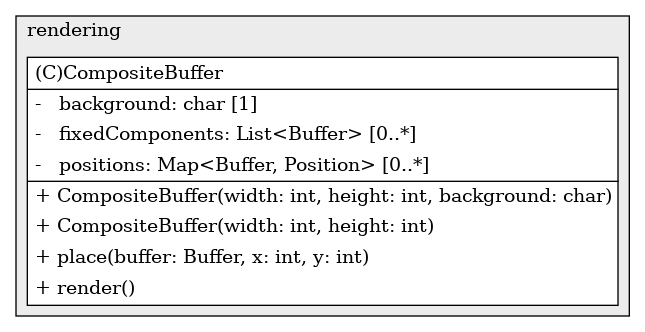
\includegraphics[width=0.6\linewidth]{Bilder/Visualisierung/CompositeBufferPlaceFunction_structure.png}
    \caption{Refactorings: Rename Method (Vorher)}
\end{figure}

\vspace{0.5cm}
\begin{lstlisting}[caption={Refactorings: Rename Method (Nachher)}]
public class CompositeBuffer extends Buffer {
    
    private final Map<Buffer, Position> fixed;
    private final char background;
    
    public CompositeBuffer(int width, int height, char background) {
        super(width, height);
        this.fixed = new LinkedHashMap<>();
        this.background = background;
    }
    
    public CompositeBuffer(int width, int height) {
        this(width, height, ' ');
    }
    
    public void fixed(Buffer buffer, int x, int y) {
        this.fixed.put(buffer, new Position(x, y));
    }
    
    public void render() {
        this.fill(this.background);
        this.color(ANSIColor.RESET);
        
        this.fixed.forEach((component, position) -> {
            component.render();
            this.write(position, component);
        });
    }
    
}
\end{lstlisting}

\vspace{0.5cm}
\begin{figure}[H]
    \centering
    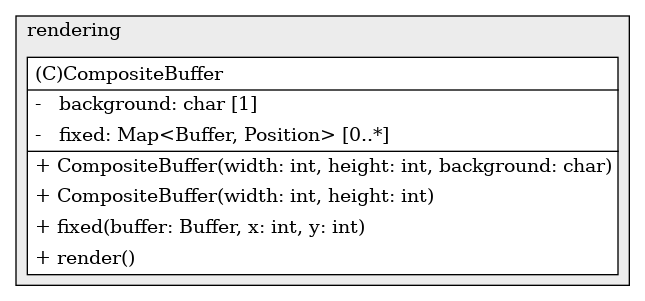
\includegraphics[width=0.6\linewidth]{Bilder/Visualisierung/CompositeBufferFixedFunction_structure.png}
    \caption{Refactorings: Rename Method (Nachher)}
\end{figure}
